\section{Highest Locker Priority}

\subsection{Definition}

 Highest Locker Priority (HLP) is the improvement of the previous protocol to allow the highest priority task $\tau_{i}$ that doesn't use resource $R_{k}$ to interrupt the lower priority task $\tau_{j}$ that use the resource, $R_{k}$ by limiting the raised priority of task $\tau_{j}$. So,
 
\begin{center}
 $p_{i}(R_{k})=\underset{h}{\mathrm{max}} \{P_{h}| \tau_{h}$ uses $R_{k}\}  $ 
\end{center}

This dynamic priority then set back to its nominal value $P_{i}$ when the task leave its critical section. The maximum raised priority of task $\tau_{j}$ is called priority ceiling $ C(R_{k}) $ and computed off-line.  The maximum priority $ C(R_{k}) $ of the tasks sharing $ R_{k} $ is the computed online such

\begin{center}
$C(R_{k})\stackrel{def}{=}\underset{h}{\mathrm{max}} \{P_{h}| \tau_{h}$ uses $R_{k}\}  $
\end{center}

Since the priority of lower priority task $\tau_{j}$ is raised as soon as the task entering $ R_{k} $, this protocol also known as Immediate Priority Ceiling. This protocol can be visualize as in \ref{fig: Example_of_schedule_under_HLP} where task $ \tau_{1} $ have higest priority and task $ \tau_{3} $ is the first task arrive

\begin{figure}[h]
    \centering
    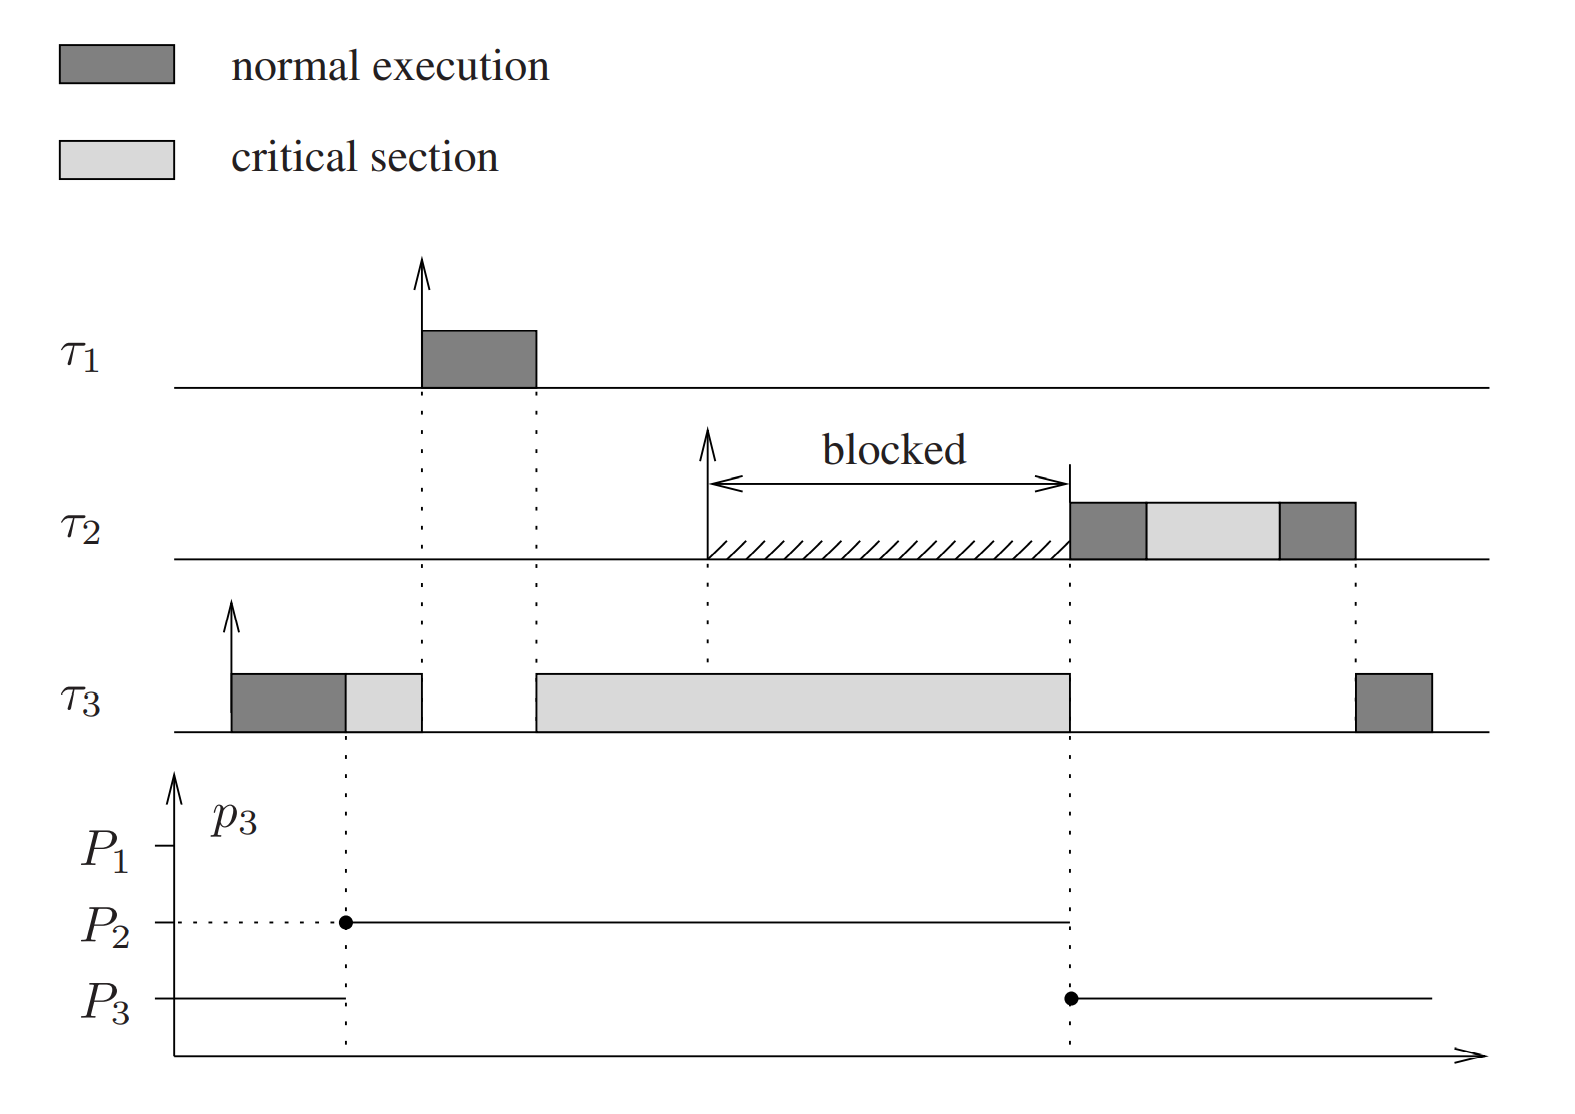
\includegraphics[width=0.5\textwidth]{Example_of_schedule_under_HLP}
    \caption{ Example of schedule under HLP, where $ p3 $ is raised at the level $ C(R) = P_{2} $ as soon as $ \tau_{3} $ starts using resource R \cite{b5}}
    \label{fig:Example_of_schedule_under_HLP}
\end{figure}

 
\subsection{Blocking Time Computation}

So, total of critical section of lower priority task $\tau_{j}$ blocking higher priority task $\tau_{i}$ is reduced by adding new parameter as shown below.

\begin{center}
$ \gamma_{i}=\{Z_{j,k} | P_{j}<P_{i} $ and $ C(R_{k})\geq P_{i} \} $
\end{center}

According to \cite{b5} - Under HLP, a task $ \tau_{i} $ can be blocked, at most, for the duration of a single critical section belonging to the set $ \gamma_{i} $ and this theorem is proved by contradiction, assuming that $ \tau_{i} $ is blocked by two critical sections, $ z_{1,a} $ and $ z_{2,b} $. For this to happen, both critical sections must belong to different tasks ($ \tau_{1} $ and $ \tau_{2} $) with priority lower than $ P_{i} $, and both must have a ceiling higher than or equal to $ P_{i} $. That is, by assumption, we must have

\begin{center}
$ P_{1}< P_{i}\leq C(R_{a})$

$ P_{2}< P_{i}\leq C(R_{b})$
\end{center}

Now, $ \tau_{i} $  can be blocked twice only if $ \tau_{1} $  and $ \tau_{2} $  are both inside the resources when $ \tau_{i} $ arrives, and this can occur only if one of them (say $ \tau_{1} $ ) preempted the other inside the critical section. But, if $ \tau_{1} $  preempted $ \tau_{2} $ inside $ z_{2,b} $  it means that $ P_{2}> C(R_{b}) $ , which is a contradiction. Hence, the theorem follows.

As shown in figure \ref{fig:Example_of_schedule_under_HLP}, $ \tau_{i} $ can be block at maximum once, means that

\begin{center}
$B_{i}(R_{k})=\underset{j,k}{\mathrm{max}} \{ \delta_{j,k}-1 | Z_{j,k} \in \gamma_{i}\}  $
\end{center}

We need to minus one unit of time because the lower priority task $ \tau_{j} $ need to access $ R_{k} $ atleast one unit time earlier then $ \tau_{i} $ to block it.

\subsection{Problem Arise}

Despite the fact that this algorithm improve the previous algorithm, it still could produce some unnecessary blocking. This algorithm block a task at the time it attempt, before it actually require a resource \cite{b5}. It also says that - If a critical section is contained only in one branch of a conditional statement, then the task could be unnecessarily blocked, since during execution it could take the branch without the resource.

This protocol was improved by Priority Inheritance protocol that will be expalain in the next section.
 










